\documentclass{article}\usepackage[]{graphicx}\usepackage[]{xcolor}
% maxwidth is the original width if it is less than linewidth
% otherwise use linewidth (to make sure the graphics do not exceed the margin)
\makeatletter
\def\maxwidth{ %
  \ifdim\Gin@nat@width>\linewidth
    \linewidth
  \else
    \Gin@nat@width
  \fi
}
\makeatother

\definecolor{fgcolor}{rgb}{0.345, 0.345, 0.345}
\newcommand{\hlnum}[1]{\textcolor[rgb]{0.686,0.059,0.569}{#1}}%
\newcommand{\hlstr}[1]{\textcolor[rgb]{0.192,0.494,0.8}{#1}}%
\newcommand{\hlcom}[1]{\textcolor[rgb]{0.678,0.584,0.686}{\textit{#1}}}%
\newcommand{\hlopt}[1]{\textcolor[rgb]{0,0,0}{#1}}%
\newcommand{\hlstd}[1]{\textcolor[rgb]{0.345,0.345,0.345}{#1}}%
\newcommand{\hlkwa}[1]{\textcolor[rgb]{0.161,0.373,0.58}{\textbf{#1}}}%
\newcommand{\hlkwb}[1]{\textcolor[rgb]{0.69,0.353,0.396}{#1}}%
\newcommand{\hlkwc}[1]{\textcolor[rgb]{0.333,0.667,0.333}{#1}}%
\newcommand{\hlkwd}[1]{\textcolor[rgb]{0.737,0.353,0.396}{\textbf{#1}}}%
\let\hlipl\hlkwb

\usepackage{framed}
\makeatletter
\newenvironment{kframe}{%
 \def\at@end@of@kframe{}%
 \ifinner\ifhmode%
  \def\at@end@of@kframe{\end{minipage}}%
  \begin{minipage}{\columnwidth}%
 \fi\fi%
 \def\FrameCommand##1{\hskip\@totalleftmargin \hskip-\fboxsep
 \colorbox{shadecolor}{##1}\hskip-\fboxsep
     % There is no \\@totalrightmargin, so:
     \hskip-\linewidth \hskip-\@totalleftmargin \hskip\columnwidth}%
 \MakeFramed {\advance\hsize-\width
   \@totalleftmargin\z@ \linewidth\hsize
   \@setminipage}}%
 {\par\unskip\endMakeFramed%
 \at@end@of@kframe}
\makeatother

\definecolor{shadecolor}{rgb}{.97, .97, .97}
\definecolor{messagecolor}{rgb}{0, 0, 0}
\definecolor{warningcolor}{rgb}{1, 0, 1}
\definecolor{errorcolor}{rgb}{1, 0, 0}
\newenvironment{knitrout}{}{} % an empty environment to be redefined in TeX

\usepackage{alltt}
\usepackage[sc]{mathpazo}
\renewcommand{\sfdefault}{lmss}
\renewcommand{\ttdefault}{lmtt}
\usepackage[T1]{fontenc}
\usepackage{geometry}
\geometry{verbose,tmargin=2.5cm,bmargin=2.5cm,lmargin=2.5cm,rmargin=2.5cm}
\setcounter{secnumdepth}{2}
\setcounter{tocdepth}{2}
\usepackage[unicode=true,pdfusetitle,
 bookmarks=true,bookmarksnumbered=true,bookmarksopen=true,bookmarksopenlevel=2,
 breaklinks=false,pdfborder={0 0 1},backref=false,colorlinks=false]
 {hyperref}
\hypersetup{
 pdfstartview={XYZ null null 1}}

\makeatletter
%%%%%%%%%%%%%%%%%%%%%%%%%%%%%% User specified LaTeX commands.
\renewcommand{\textfraction}{0.05}
\renewcommand{\topfraction}{0.8}
\renewcommand{\bottomfraction}{0.8}
\renewcommand{\floatpagefraction}{0.75}

\makeatother
\IfFileExists{upquote.sty}{\usepackage{upquote}}{}
\begin{document}








The results below are generated from an R script.

\begin{knitrout}
\definecolor{shadecolor}{rgb}{0.969, 0.969, 0.969}\color{fgcolor}\begin{kframe}
\begin{alltt}
\hlcom{#Question 1}
\hlkwd{library}\hlstd{(DAAG)}
\hlcom{#a. }
\hlkwd{par}\hlstd{(}\hlkwc{mar} \hlstd{=} \hlkwd{c}\hlstd{(}\hlnum{5}\hlstd{,} \hlnum{5}\hlstd{,} \hlnum{4}\hlstd{,} \hlnum{2}\hlstd{)} \hlopt{+} \hlnum{0.1}\hlstd{)}
\hlkwd{plot}\hlstd{(Manitoba.lakes,} \hlkwc{xlim}\hlstd{=} \hlkwd{c}\hlstd{(}\hlnum{160}\hlstd{,}\hlnum{260}\hlstd{),}\hlkwc{cex}\hlstd{=}\hlnum{0.7}\hlstd{)}
\hlcom{#b. }
\hlkwd{text}\hlstd{(Manitoba.lakes,} \hlkwc{labels}\hlstd{=}\hlkwd{rownames}\hlstd{(Manitoba.lakes),} \hlkwc{cex}\hlstd{=}\hlnum{0.7}\hlstd{,} \hlkwc{pos}\hlstd{=} \hlnum{2}\hlstd{)}
\hlcom{#c.}
\hlstd{myPlot} \hlkwb{=} \hlkwd{lm}\hlstd{(area} \hlopt{~} \hlstd{elevation,} \hlkwc{data}\hlstd{=Manitoba.lakes)}
\hlkwd{abline}\hlstd{(myPlot,} \hlkwc{col}\hlstd{=}\hlstr{"blue"}\hlstd{)}
\end{alltt}
\end{kframe}

{\centering 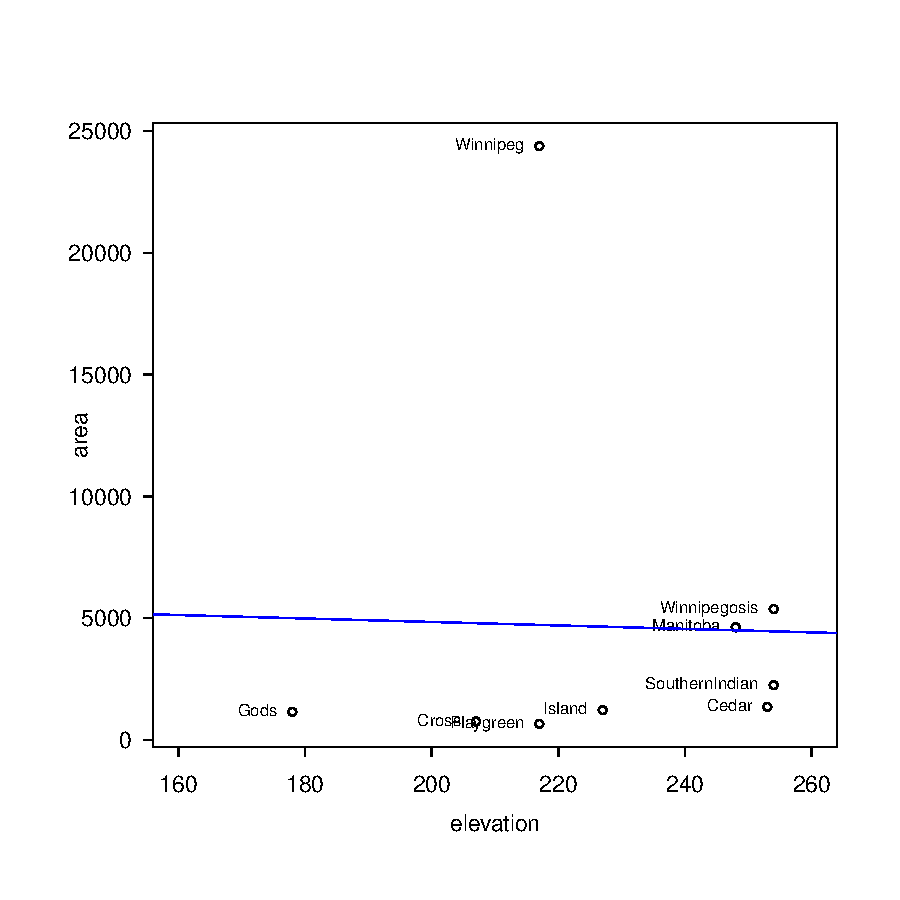
\includegraphics[width=.6\linewidth]{figure/Meng51940633A3-Rnwauto-report-1} 

}


\begin{kframe}\begin{alltt}
\hlcom{#d.}
\hlstd{elevationdivided1000} \hlkwb{=} \hlstd{Manitoba.lakes}\hlopt{$}\hlstd{elevation}\hlopt{/}\hlnum{1000}
\hlstd{areadivided100} \hlkwb{=} \hlstd{Manitoba.lakes}\hlopt{$}\hlstd{area}\hlopt{/}\hlnum{100}
\hlstd{ML.df} \hlkwb{=} \hlkwd{data.frame}\hlstd{(elevationdivided1000,areadivided100)}
\hlkwd{plot}\hlstd{(ML.df)}
\end{alltt}
\end{kframe}

{\centering 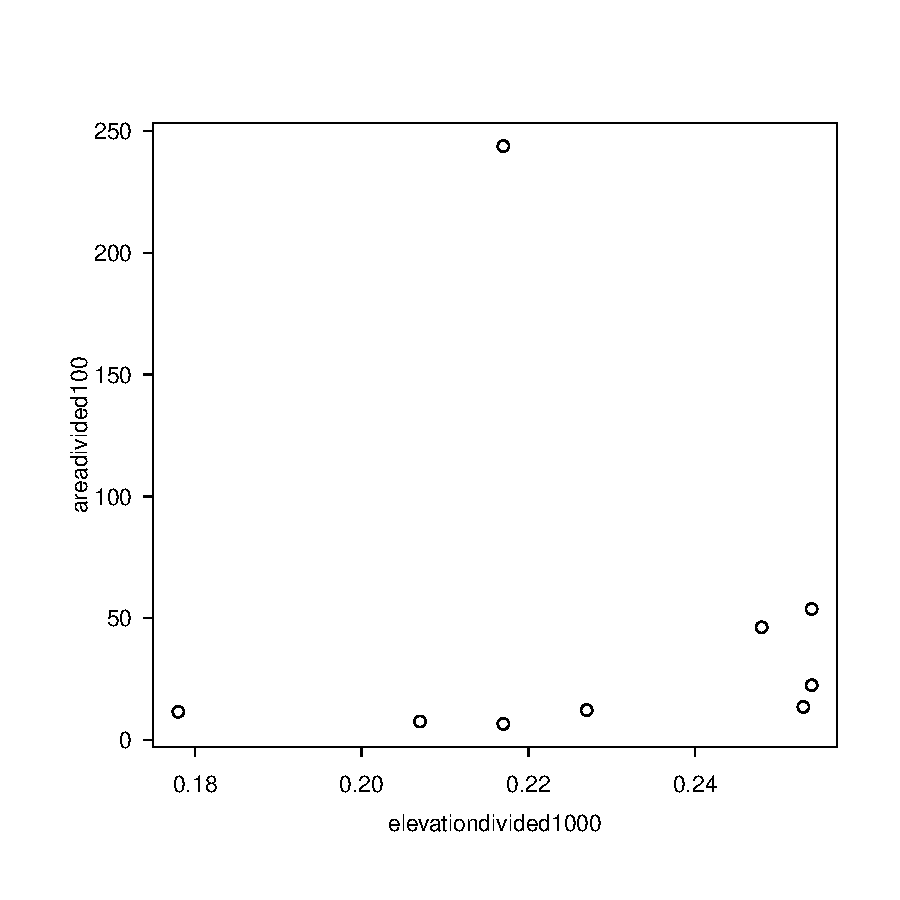
\includegraphics[width=.6\linewidth]{figure/Meng51940633A3-Rnwauto-report-2} 

}


\begin{kframe}\begin{alltt}
\hlcom{# redo for areadivided1000 and elevationdivided100 }
\hlstd{elevationdivided100} \hlkwb{=} \hlstd{Manitoba.lakes}\hlopt{$}\hlstd{elevation}\hlopt{/}\hlnum{100}
\hlstd{areadivided1000} \hlkwb{=} \hlstd{Manitoba.lakes}\hlopt{$}\hlstd{area}\hlopt{/}\hlnum{1000}
\hlstd{ML.df} \hlkwb{=} \hlkwd{data.frame}\hlstd{(elevationdivided100,areadivided1000)}
\hlkwd{plot}\hlstd{(ML.df)}
\end{alltt}
\end{kframe}

{\centering 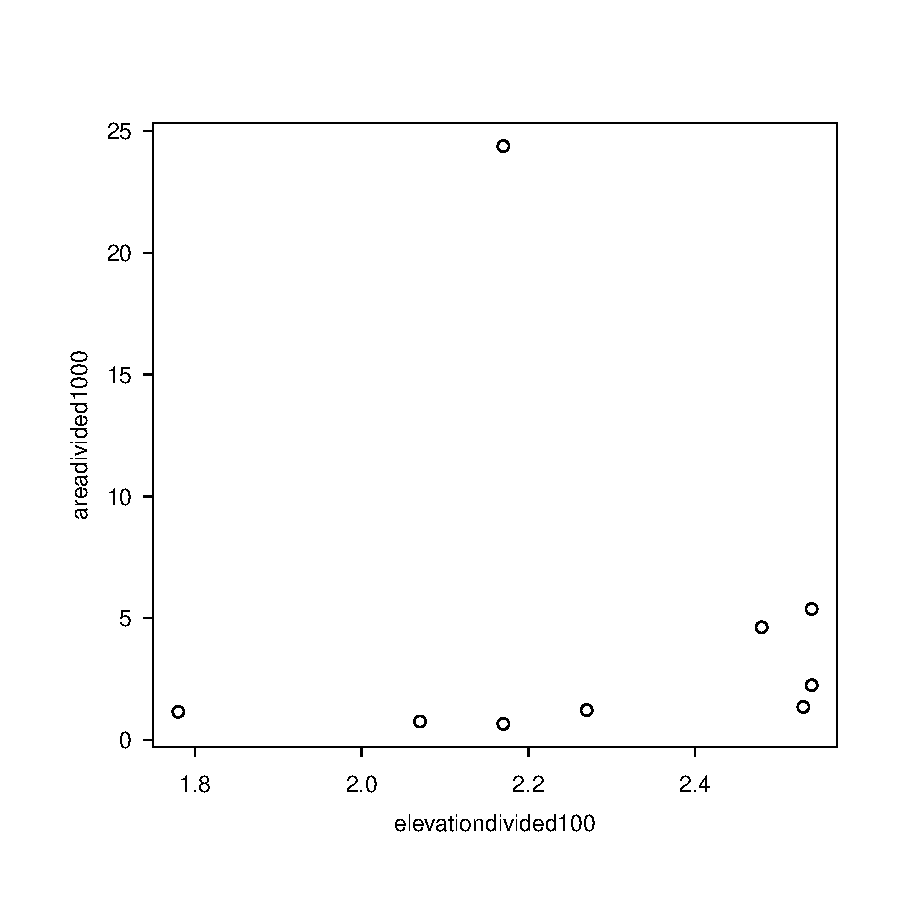
\includegraphics[width=.6\linewidth]{figure/Meng51940633A3-Rnwauto-report-3} 

}


\begin{kframe}\begin{alltt}
\hlcom{#Question 2}
\hlkwd{help}\hlstd{(unique)}
\hlstd{myData} \hlkwb{=} \hlkwd{c}\hlstd{(}\hlnum{1}\hlstd{,}\hlnum{1}\hlstd{,}\hlnum{1}\hlstd{,}\hlnum{2}\hlstd{,}\hlnum{3}\hlstd{,}\hlnum{4}\hlstd{,}\hlnum{4}\hlstd{,}\hlnum{5}\hlstd{,}\hlnum{5}\hlstd{,}\hlnum{6}\hlstd{,}\hlnum{6}\hlstd{,}\hlnum{6}\hlstd{,}\hlnum{6}\hlstd{,}\hlnum{7}\hlstd{)}
\hlkwd{unique}\hlstd{(myData)}
\end{alltt}
\begin{verbatim}
## [1] 1 2 3 4 5 6 7
\end{verbatim}
\begin{alltt}
\hlcom{#unique takes data that is not repeated and returns it.}
\hlkwd{unique}\hlstd{(myData,} \hlkwc{incomparables} \hlstd{=} \hlnum{1}\hlstd{)}
\end{alltt}
\begin{verbatim}
## [1] 1 1 1 2 3 4 5 6 7
\end{verbatim}
\begin{alltt}
\hlcom{#incomparables means that it will not compare whatever value is given, for example here,}
\hlcom{#this will return all 1's.}

\hlcom{#Question 3}
\hlkwd{plot}\hlstd{(Loblolly}\hlopt{$}\hlstd{age, Loblolly}\hlopt{$}\hlstd{height,} \hlkwc{xlab}\hlstd{=}\hlstr{"age"}\hlstd{,} \hlkwc{ylab}\hlstd{=}\hlstr{"height"}\hlstd{,} \hlkwc{main}\hlstd{=}\hlstr{"height vs age"}\hlstd{)}
\hlkwd{abline}\hlstd{(}\hlkwd{lm}\hlstd{(height}\hlopt{~}\hlstd{age,} \hlkwc{data}\hlstd{=Loblolly),} \hlkwc{col}\hlstd{=}\hlstr{"red"}\hlstd{)}
\end{alltt}
\end{kframe}

{\centering 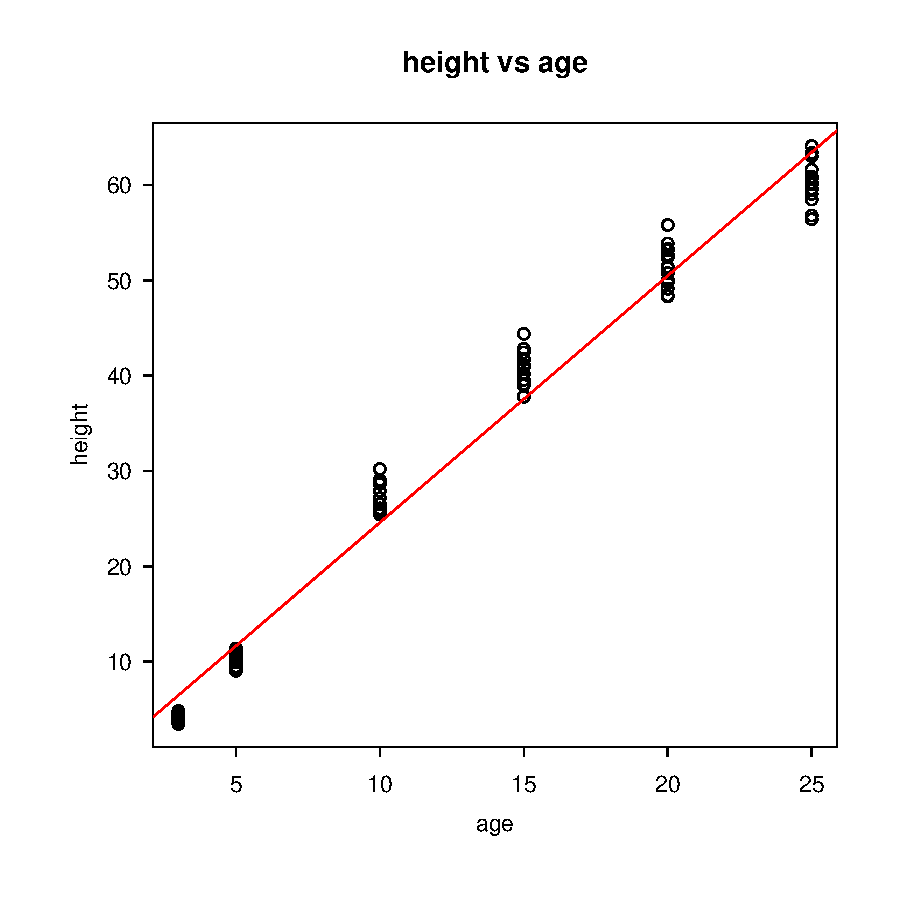
\includegraphics[width=.6\linewidth]{figure/Meng51940633A3-Rnwauto-report-4} 

}


\begin{kframe}\begin{alltt}
\hlcom{#Question 4}
\hlcom{# I believe this data is believable because if we think about it the older the pine tree}
\hlcom{# the higher the tree but loblolly reaches its maximum height in around 150 years, so this}
\hlcom{# data is true for now.}

\hlcom{#Question 5}
\hlstd{returns1} \hlkwb{=} \hlkwd{diff}\hlstd{(EuStockMarkets)}
\hlkwd{hist}\hlstd{(returns1)}
\end{alltt}
\end{kframe}

{\centering 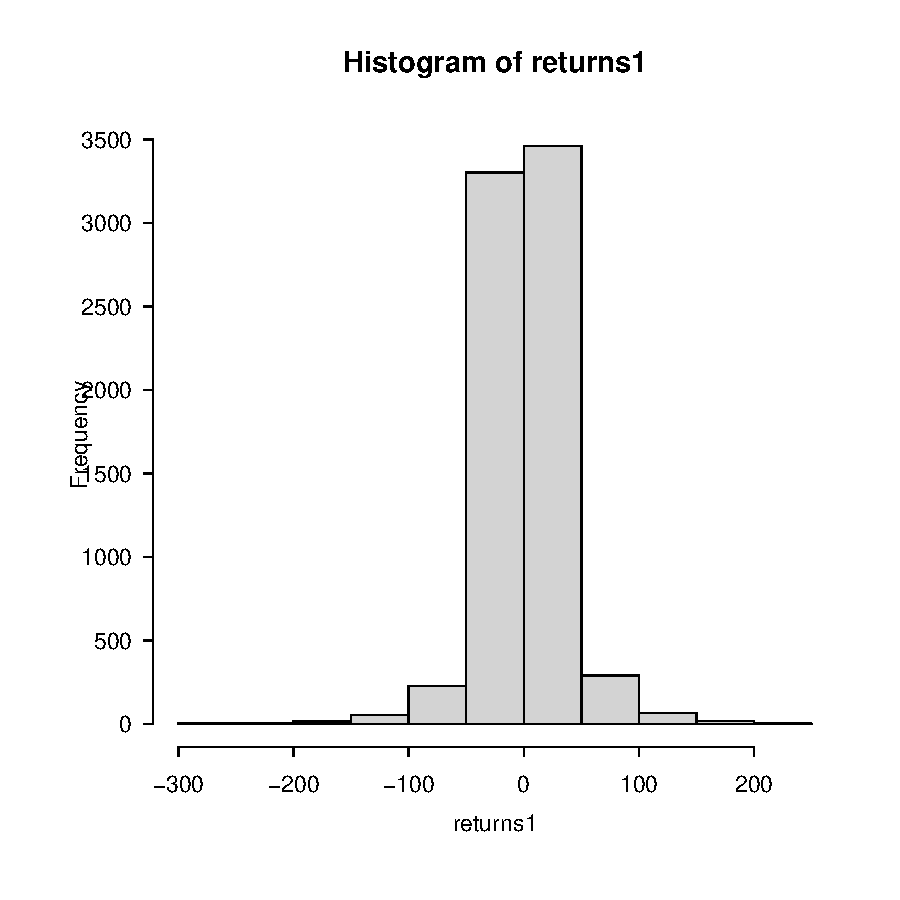
\includegraphics[width=.6\linewidth]{figure/Meng51940633A3-Rnwauto-report-5} 

}


\begin{kframe}\begin{alltt}
\hlkwd{hist}\hlstd{(returns1,} \hlkwc{breaks} \hlstd{=} \hlstr{"scott"}\hlstd{)}
\hlkwd{hist}\hlstd{(returns1,} \hlkwc{breaks} \hlstd{=} \hlstr{"fd"}\hlstd{)}
\end{alltt}
\end{kframe}

{\centering 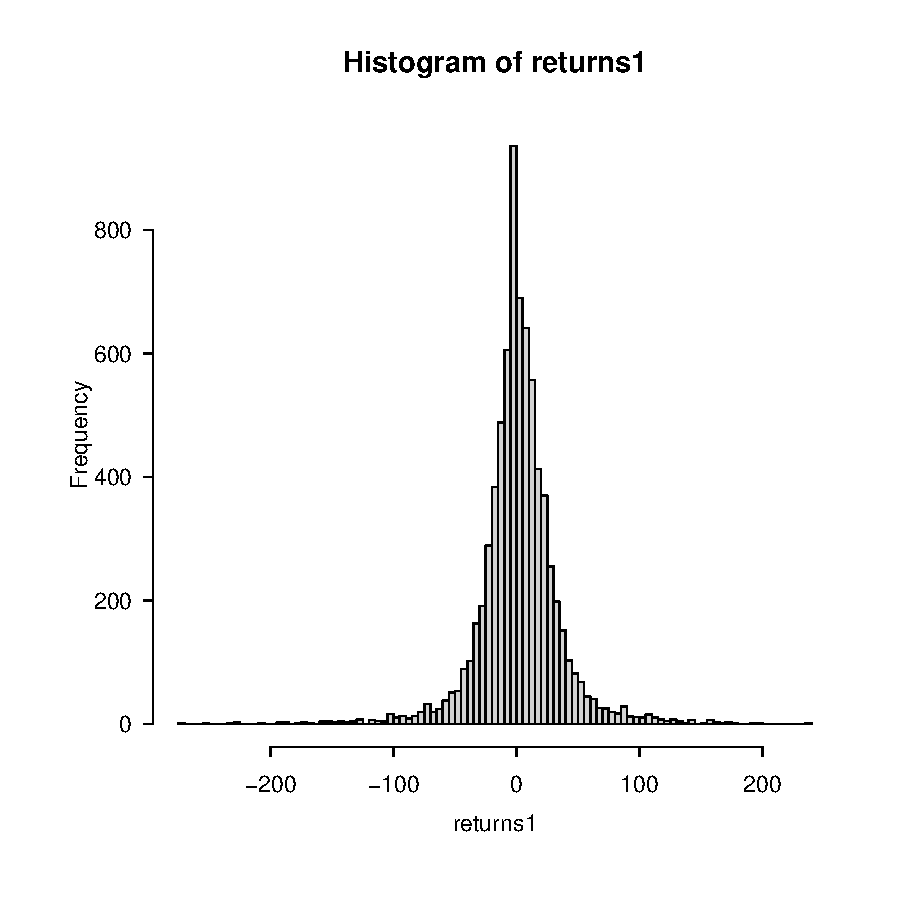
\includegraphics[width=.6\linewidth]{figure/Meng51940633A3-Rnwauto-report-6} 

}


\begin{kframe}\begin{alltt}
\hlcom{# they both look the same}

\hlcom{#Question 6}

\hlcom{# create points for b.}
\hlstd{x} \hlkwb{<-} \hlkwd{c}\hlstd{(}\hlnum{8}\hlstd{,} \hlnum{10}\hlstd{,} \hlnum{15}\hlstd{,} \hlnum{11}\hlstd{,} \hlnum{12.5}\hlstd{,} \hlnum{8.5}\hlstd{,} \hlnum{4}\hlstd{,} \hlnum{6}\hlstd{,} \hlnum{2}\hlstd{,} \hlnum{7}\hlstd{,} \hlnum{8}\hlstd{)}
\hlstd{y} \hlkwb{<-} \hlkwd{c}\hlstd{(}\hlnum{15}\hlstd{,} \hlnum{10}\hlstd{,} \hlnum{10}\hlstd{,} \hlnum{7}\hlstd{,} \hlnum{2}\hlstd{,} \hlnum{5}\hlstd{,} \hlnum{2}\hlstd{,} \hlnum{7}\hlstd{,} \hlnum{10}\hlstd{,} \hlnum{10}\hlstd{,} \hlnum{15}\hlstd{)}
\hlstd{pointNames} \hlkwb{=} \hlkwd{c}\hlstd{(}\hlstr{"A"}\hlstd{,}\hlstr{"B"}\hlstd{,}\hlstr{"C"}\hlstd{,}\hlstr{"D"}\hlstd{,}\hlstr{"E"}\hlstd{,}\hlstr{"F"}\hlstd{,}\hlstr{"G"}\hlstd{,}\hlstr{"H"}\hlstd{,}\hlstr{"I"}\hlstd{,}\hlstr{"J"}\hlstd{)}

\hlcom{# c.}
\hlkwd{par}\hlstd{(}\hlkwc{mar} \hlstd{=} \hlkwd{c}\hlstd{(}\hlnum{4}\hlstd{,} \hlnum{4}\hlstd{,} \hlnum{4}\hlstd{,} \hlnum{4}\hlstd{),} \hlkwc{pin} \hlstd{=} \hlkwd{c}\hlstd{(}\hlnum{4}\hlstd{,} \hlnum{4}\hlstd{),}\hlkwc{bg}\hlstd{=}\hlstr{"blue"}\hlstd{)}
\hlstd{mystar} \hlkwb{=} \hlkwd{plot}\hlstd{(x,y,} \hlkwc{asp} \hlstd{=} \hlnum{1}\hlstd{,} \hlkwc{cex} \hlstd{=} \hlnum{0.7}\hlstd{,} \hlkwc{xlim} \hlstd{=}\hlkwd{c}\hlstd{(}\hlnum{2}\hlstd{,}\hlnum{15}\hlstd{),} \hlkwc{ylim} \hlstd{=} \hlkwd{c}\hlstd{(}\hlnum{2}\hlstd{,}\hlnum{15}\hlstd{))}
\hlkwd{text}\hlstd{(x,y,}\hlkwc{labels} \hlstd{= pointNames,}\hlkwc{pos}\hlstd{=}\hlnum{2}\hlstd{,}\hlkwc{cex} \hlstd{=} \hlnum{0.7}\hlstd{)}
\hlkwd{lines}\hlstd{(x,y,} \hlkwc{col} \hlstd{=} \hlstr{"red"}\hlstd{,}\hlkwc{lwd} \hlstd{=} \hlnum{3}\hlstd{)}
\end{alltt}
\end{kframe}

{\centering 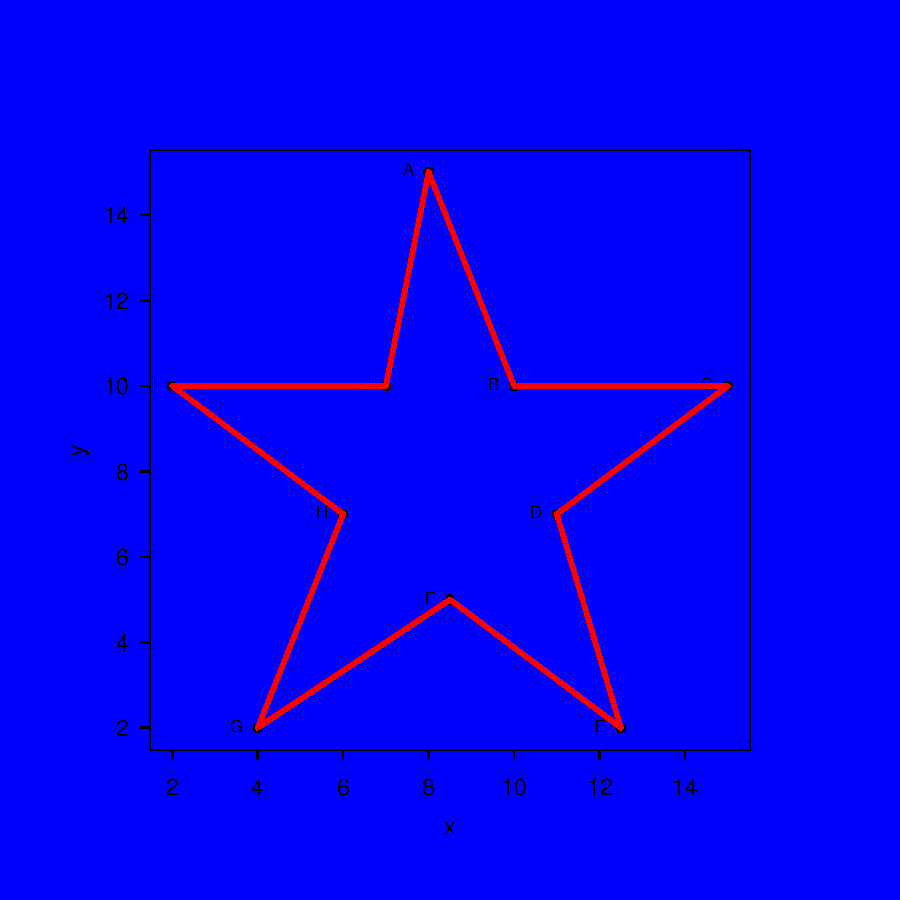
\includegraphics[width=.6\linewidth]{figure/Meng51940633A3-Rnwauto-report-7} 

}


\begin{kframe}\begin{alltt}
\hlcom{#BONUS}
\hlstd{mystar} \hlkwb{=} \hlkwd{plot}\hlstd{(x,y,} \hlkwc{asp} \hlstd{=} \hlnum{1}\hlstd{,} \hlkwc{cex} \hlstd{=} \hlnum{0.7}\hlstd{,} \hlkwc{xlim} \hlstd{=}\hlkwd{c}\hlstd{(}\hlnum{2}\hlstd{,}\hlnum{15}\hlstd{),} \hlkwc{ylim} \hlstd{=} \hlkwd{c}\hlstd{(}\hlnum{2}\hlstd{,}\hlnum{15}\hlstd{),} \hlkwc{type}\hlstd{=}\hlstr{"n"}\hlstd{)}
\hlkwd{polygon}\hlstd{(x,y,}\hlkwc{col}\hlstd{=}\hlstr{"yellow"}\hlstd{)}
\hlkwd{text}\hlstd{(}\hlnum{8.5}\hlstd{,}\hlnum{8}\hlstd{,}\hlkwc{labels} \hlstd{=} \hlstr{"MY STAR"}\hlstd{,} \hlkwc{col}\hlstd{=} \hlstr{"blue"}\hlstd{,} \hlkwc{cex} \hlstd{=} \hlnum{1.5}\hlstd{)}
\end{alltt}
\end{kframe}

{\centering 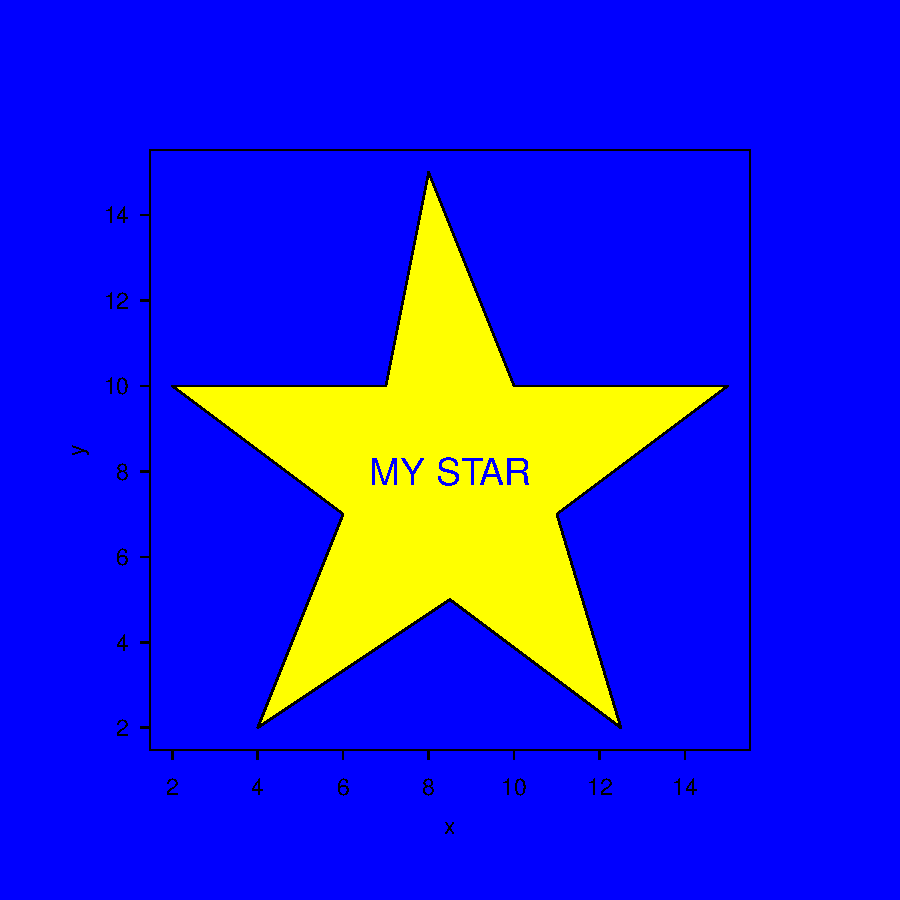
\includegraphics[width=.6\linewidth]{figure/Meng51940633A3-Rnwauto-report-8} 

}


\end{knitrout}

The R session information (including the OS info, R version and all
packages used):

\begin{knitrout}
\definecolor{shadecolor}{rgb}{0.969, 0.969, 0.969}\color{fgcolor}\begin{kframe}
\begin{alltt}
\hlkwd{sessionInfo}\hlstd{()}
\end{alltt}
\begin{verbatim}
## R version 4.2.2 (2022-10-31)
## Platform: x86_64-apple-darwin17.0 (64-bit)
## Running under: macOS Ventura 13.1
## 
## Matrix products: default
## LAPACK: /Library/Frameworks/R.framework/Versions/4.2/Resources/lib/libRlapack.dylib
## 
## locale:
## [1] en_US.UTF-8/en_US.UTF-8/en_US.UTF-8/C/en_US.UTF-8/en_US.UTF-8
## 
## attached base packages:
## [1] stats     graphics  grDevices utils     datasets  methods   base     
## 
## other attached packages:
## [1] DAAG_1.25.4
## 
## loaded via a namespace (and not attached):
##  [1] Rcpp_1.0.10         lattice_0.20-45     deldir_1.0-6        png_0.1-8          
##  [5] rbibutils_2.2.13    grid_4.2.2          evaluate_0.20       highr_0.10         
##  [9] Rdpack_2.4          latticeExtra_0.6-30 RColorBrewer_1.1-3  tools_4.2.2        
## [13] interp_1.1-3        jpeg_0.1-10         xfun_0.37           compiler_4.2.2     
## [17] knitr_1.42
\end{verbatim}
\begin{alltt}
\hlkwd{Sys.time}\hlstd{()}
\end{alltt}
\begin{verbatim}
## [1] "2023-03-28 10:49:42 PDT"
\end{verbatim}
\end{kframe}
\end{knitrout}


\end{document}
